\documentclass{article}

\usepackage{graphicx}
\usepackage{tikz}
\usepackage{tikzsymbols}
\usetikzlibrary{calc,patterns,shapes.geometric}
\pagestyle{empty}
\usepackage[margin=0pt]{geometry}
\geometry{papersize={14in,12in}}

\def\centerarc[#1](#2)(#3:#4:#5){\draw[#1] ($(#2)+({#5*cos(#3)},{#5*sin(#3)})$) arc (#3:#4:#5);}

\begin{document}
	\begin{figure}
		\centering
		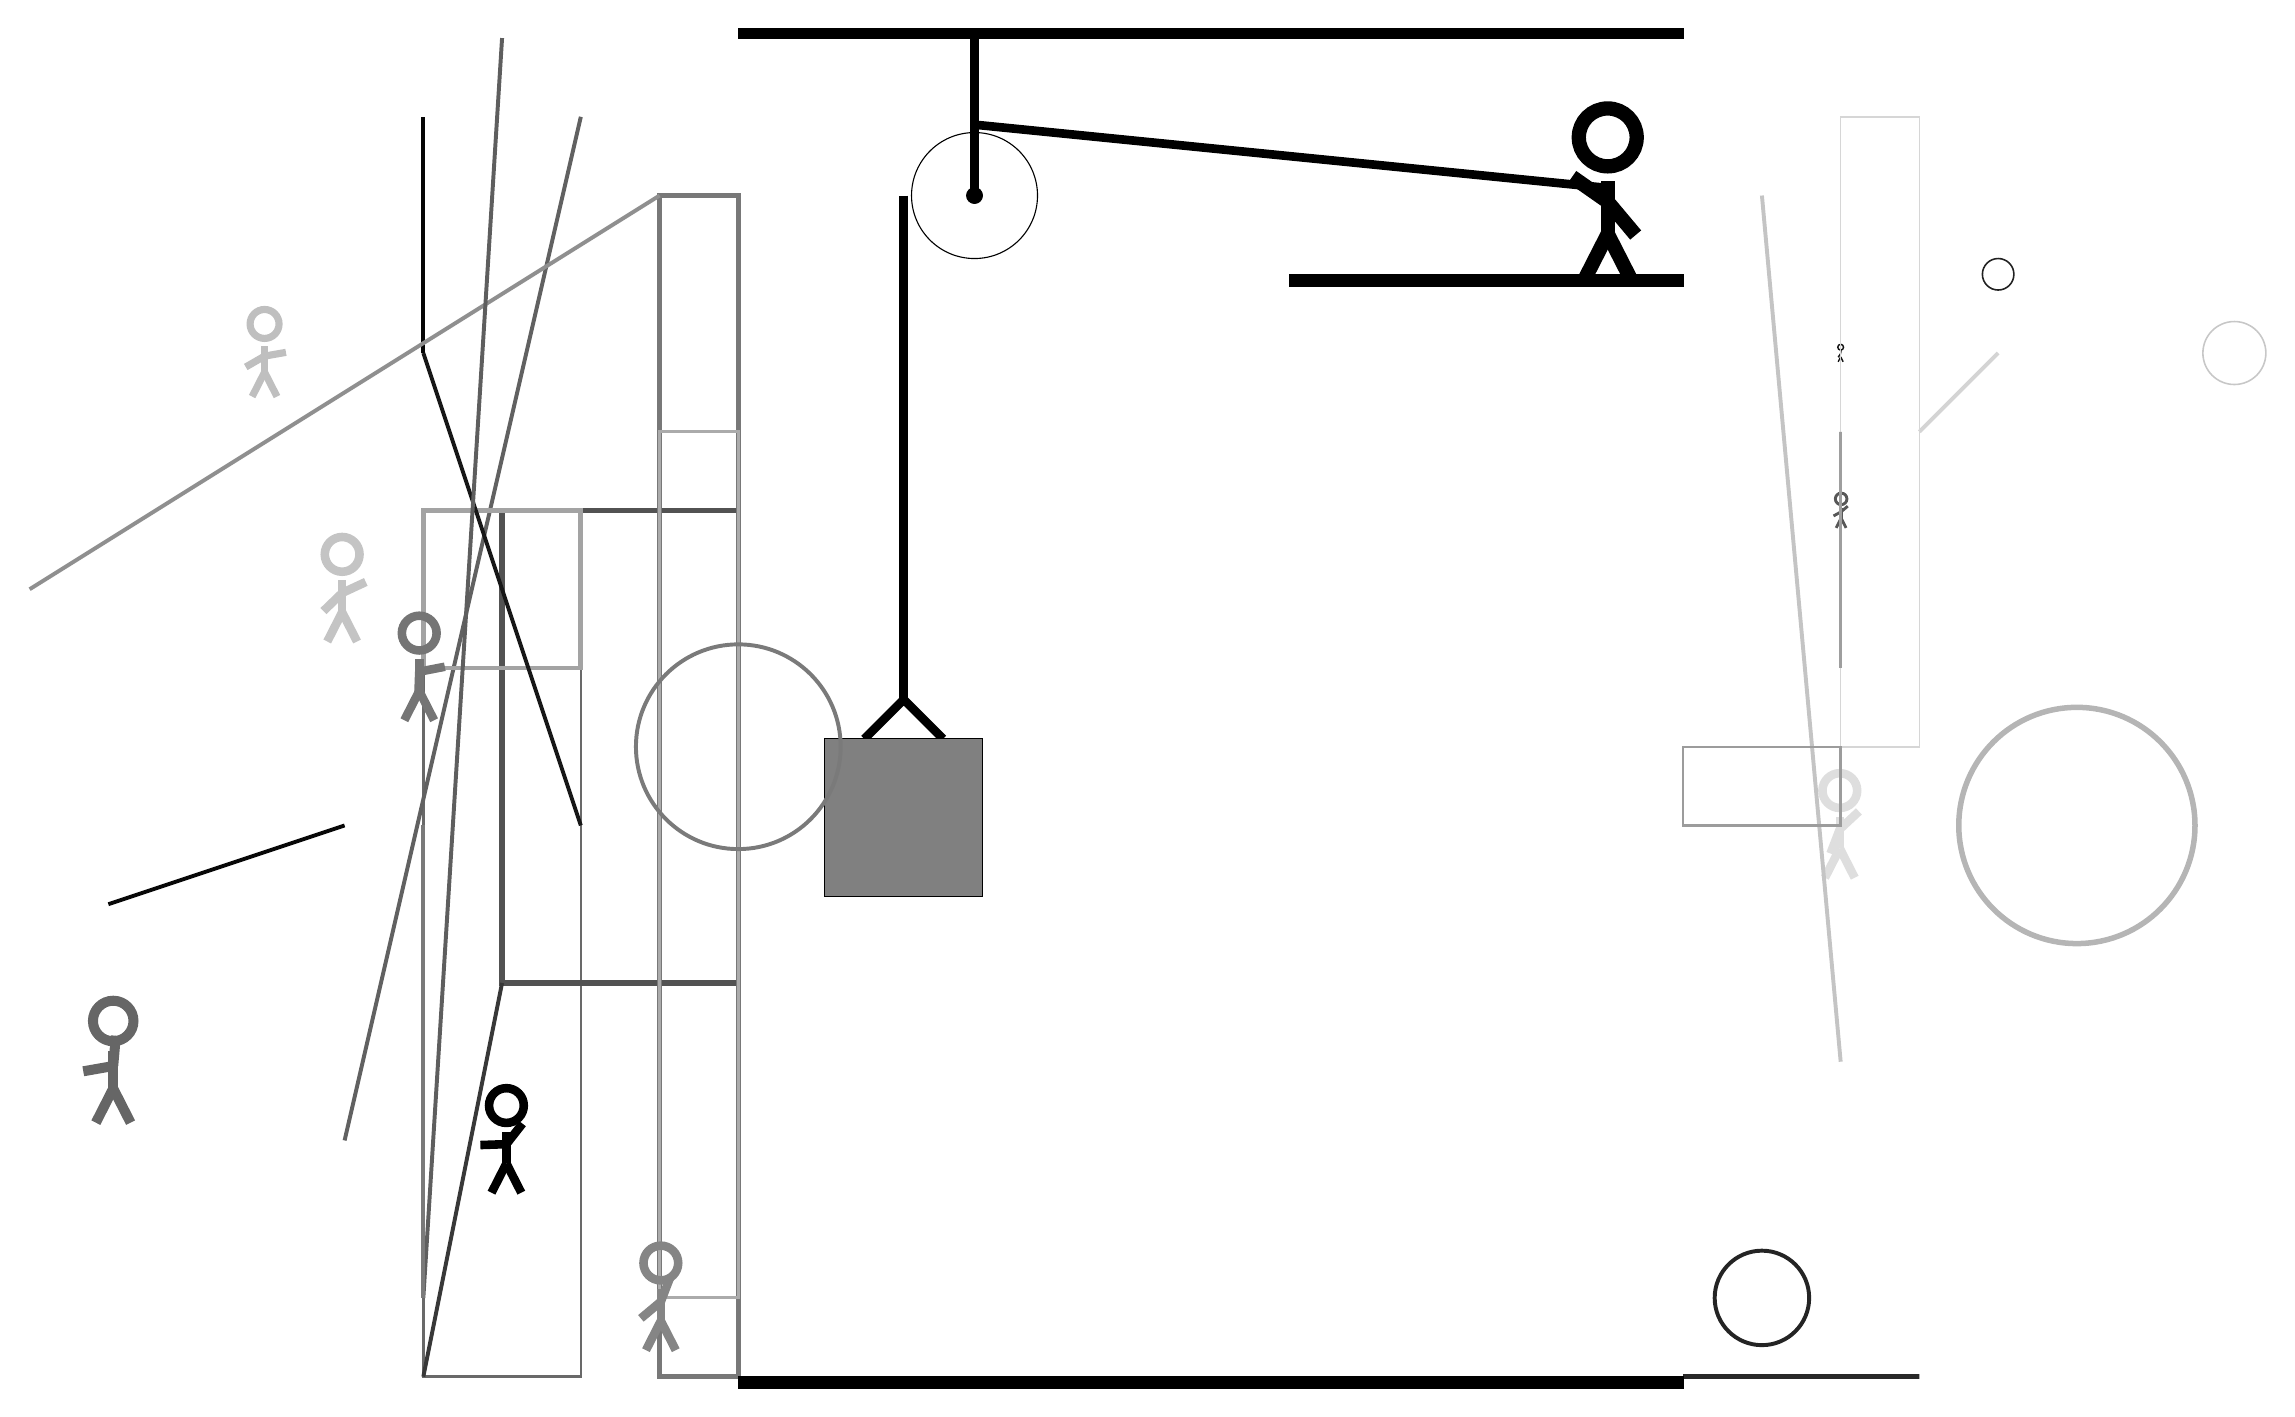
\begin{tikzpicture}
			%%%%% START %%%%%
			
			\draw[fill=black] (-2, 14) rectangle (10, 14.125);
			
			\draw (1, 12) circle (0.8);
			\draw[fill=black] (1, 12) circle (0.1);
			\draw[line width=1.1mm] (1, 14) -- (1, 12);
			
			\draw[line width=1.1mm](-0.4, 5.1) --  (0.1, 5.6) -- (0.6, 5.1);
			\draw[fill=black!50] (-0.9, 5.1) rectangle (1.1, 3.1);
			
			\draw [line width=0.5mm, color=black!86](11, -2) circle (0.6);
			
			\draw[line width=0.3mm, color=black!59] (-4, -3) rectangle (-6, 6);
			\draw[line width=0.5mm, color=black!62](-7, 0) -- (-4, 13);
			\node[line width=0.5mm, color=black!60] at (-10, 1) {\Strichmaxerl[7][10][85]};
			
			\draw[line width=0.5mm, color=black!98](-6, 10) -- (-6, 13);
			
			\node[line width=0.6mm, color=black!25] at (-8, 10) {\Strichmaxerl[5][30][10]};
			
			\draw[line width=0.7mm, color=black!68] (-2, 8) rectangle (-5, 2);
			
			\draw[line width=0.6mm, color=black!36] (-4, 8) rectangle (-6, 6);
			\draw[line width=0.2mm, color=black!75] (-3, 13) rectangle (-3, 13);
			
			\draw[line width=0.7mm, color=black!53] (-2, -3) rectangle (-3, 12);
			\node[line width=0.6mm, color=black!100] at (-5, 0) {\Strichmaxerl[6][2][52]};
			
			\draw[line width=0.7mm, color=black!84] (10, -3) rectangle (13, -3);
			\draw [line width=0.2mm, color=black!22](17, 10) circle (0.4);
			
			\draw [line width=0.7mm, color=black!29](15, 4) circle (1.5);
			\draw[line width=0.5mm, color=black!44](-3, 12) -- (-11, 7);
			\draw[line width=0.5mm, color=black!78](-5, 2) -- (-6, -3);
			
			\draw[line width=0.5mm, color=black!97](-7, 4) -- (-10, 3);
			
			\draw[line width=0.5mm, color=black!17](14, 10) -- (13, 9);
			\draw[line width=0.4mm, color=black!33] (-2, 9) rectangle (-3, -2);
			\node[line width=0.2mm, color=black!23] at (-7, 7) {\Strichmaxerl[6][44][25]};
			\node[line width=0.5mm, color=black!48] at (-3, -2) {\Strichmaxerl[6][40][69]};
			\node[line width=0.7mm, color=black!93] at (12, 10) {\Strichmaxerl[1][55][85]};
			
			\draw [line width=0.5mm, color=black!52](-2, 5) circle (1.3);
			\node[line width=0.4mm, color=black!66] at (12, 8) {\Strichmaxerl[2][29][40]};
			\draw[line width=0.5mm, color=black!91](-4, 4) -- (-6, 10);
			
			\node[line width=0.5mm, color=black!13] at (12, 4) {\Strichmaxerl[6][69][43]};
			\draw[line width=0.5mm, color=black!63](-5, 14) -- (-6, -2);
			\draw[line width=0.2mm, color=black!16] (12, 13) rectangle (13, 5);
			\node[line width=0.2mm, color=black!54] at (-6, 6) {\Strichmaxerl[6][88][11]};
			
			\draw[line width=0.5mm, color=black!52](-6, -2) -- (-6, 4);
			\draw[line width=0.5mm, color=black!23](11, 12) -- (12, 1);
			
			\draw[line width=0.4mm, color=black!38] (12, 9) rectangle (12, 6);
			\draw [line width=0.2mm, color=black!87](14, 11) circle (0.2);
			
			\draw[line width=0.3mm, color=black!39] (12, 5) rectangle (10, 4);
			
			\draw[line width=1.1mm](0.1, 12) -- (0.1, 5.6);
			\centerarc[line width=1.1mm](1, 12)(90:180:0.9)
			\draw[line width=1.1mm](1, 12.9) -- (9, 12.1);
			
			\node at (9, 12) {\Strichmaxerl[10][-35][-50]};
			\draw[fill=black] (5, 11) rectangle (10, 10.85);
			
			\draw[fill=black] (-2, -3) rectangle (10, -3.15);
			
			%%%%% END %%%%%
		\end{tikzpicture}
	\end{figure}	
\end{document}